% 대한산업공학회지(JKIIE) 제출용 한글 full paper (XeLaTeX + kotex)
%   xelatex jkiie_korean.tex  (2회)
% 원칙: 기술 용어는 자연스러움을 위해 영어를 그대로 사용한다.
\documentclass[10pt,a4paper]{article}
\usepackage[margin=25mm]{geometry}
\usepackage{kotex}
\usepackage{amsmath,amssymb}
\usepackage{graphicx}
\graphicspath{{figures/}}
\usepackage{float}
\usepackage{booktabs,array}
\usepackage[font=small,labelfont=bf]{caption}
\usepackage{setspace}
\setstretch{2.0}
\usepackage[hidelinks]{hyperref}
\usepackage{titlesec}
\titleformat{\section}{\Large\bfseries}{\thesection.}{0.5em}{}
\titleformat{\subsection}{\large\bfseries}{\thesubsection}{0.5em}{}
\titlespacing*{\section}{0pt}{12pt}{6pt}
\titlespacing*{\subsection}{0pt}{10pt}{4pt}
\setlength{\parindent}{1em}



\begin{document}
\begin{center}
{\Large\bfseries 도착 시각(release time)과 soft due date를 갖는 입출고 병행 트럭 크로스도킹 스케줄링: 정확해 검증을 동반한 병목 유도 반복 지역탐색}\\[2mm]
{\large Compound-Truck Cross-Docking Scheduling with Release Times and Soft Due Dates: A Bottleneck-Guided Iterated Local Search with Exact-Solver Verification}\\[4mm]
{\small 이곳에 저자명 및 소속을 넣지 마십시오. 심사 완료 후 최종본 작성 시 추가.}
\end{center}


\begin{abstract}
\noindent We study truck scheduling in a multi-door cross-dock where a compound truck is partially unloaded and then departs as an outbound carrier. Existing models assume all trucks are available at time zero and minimize makespan only. We extend the problem with per-truck release times and soft due dates (violable at a tardiness cost), minimizing makespan plus total tardiness, and formulate it as a mixed-integer program and a CP-SAT model under a reproducible seed protocol. VAA-GILS is an iterated local search combining Vogel-style construction, best-improvement descent, bottleneck-guided operators, and kick restarts. Where CP-SAT provides a reference, VAA-GILS is within 0.11–0.21% of it in under one second, versus 76–237 seconds; where optimality was proven, it averages 0.21% above the optimum. Where CP-SAT finds no feasible schedule within 600 seconds, it returns the best solutions observed. Ablation attributes the gain to this deterministic structure, not to learned operator selection.

\smallskip
\noindent\textbf{Keywords:} Cross-Docking, Compound Truck, Release Time, Soft Due Date, Iterated Local Search, Constraint Programming
\end{abstract}

\section{1. 서 론}

크로스도킹은 입고 화물을 창고에 보관하지 않고 곧바로 출고트럭으로 환적하여
재고와 리드타임을 줄이는 물류 방식이다(Boysen and Fliedner, 2010; Van Belle et al., 2012). Joo와
Kim(2013)이 도입하고 Shahmardan과 Sajadieh(2020)가
발전시킨 병행 트럭(compound truck) 변형에서는 한 대의 트럭이 두 역할을 겸한다. 여러 목적지
화물을 싣고 도착한 뒤 한 목적지의 화물은 유지하고 나머지만 \textbf{부분적으로} 하역하며,
이후 해당 목적지의 나머지 화물을 적재해 출고 운송 트럭으로 출발한다. 부분 하역은 전량 하역 대비
총 작업완료시간을 크게 줄이는 것으로 보고되어 LTL 통합 네트워크에서 실용적 매력이 크다.

기존 병행 트럭 모델의 두 가정이 현실성을 제약한다. 첫째, 모든 트럭이 시각
0에 가용하다고 가정하지만 실제 도크에서는 트럭마다 예약 도착 시각이 다르다. 둘째,
목적식이 순수 총 작업완료시간이지만 출고트럭의 출발은 위반 시 비용이 발생하는 due date에
묶여 있다.

도착 시각, 시간창(time window), 납기지연은 일반 크로스도킹 스케줄링에서 이미
연구되어 왔다(Van Belle et al., 2013; Assadi and Bagheri, 2016; Bodnar et al., 2017; Molavi et al., 2018; Rijal et al., 2019; Li et al., 2026).
그러나 병행 트럭 설정은 temporal constraint의 의미를 바꾼다. 병행 트럭은
순수 입고트럭도 출고트럭도 아니다. 부분 하역 후 한 목적지의 화물을 유지하고, 해당
목적지로 들어오는 이송 화물을 기다린 뒤 비로소 출고 운송 트럭으로 출발한다. 이 부분 하역
변환은 하나의 precedence chain --- 도착 $\to$
부분 하역 $\to$ 유지 화물 $\to$ 이송 대기 $\to$ 출고 ---
을 만들고, 이 chain은 트럭들을 공유 목적지를 통해 결합한다. 따라서 도착 시각을
추가한다고 해서 한 트럭의 시작 시각만 늦어지는 것은 아니다. 늦은 도착은 해당 트럭의
이송 화물에 의존하는 모든 출고 운송 트럭으로 전파되고, soft due date는 이 연쇄 지연을
납기지연 비용으로 바꾼다. 본 연구의 기여는 이 상호작용 --- 알려진 도착 시각과
soft due date가 부분 하역 후 출고 운송 트럭으로 전환되는 과정과 결합되는 방식 --- 을 정식화하고 분석하는
것이며, 저자가 아는 한 이 결합은 이전에 모형화된 바 없다.

본 논문의 기여는 세 가지다. 첫째, 부분 하역 병행 트럭 스케줄링을 트럭별
도착 시각과 soft due date를 갖는 문제로 확장하고, 이를 독립적인 스케줄 평가기와
일치하는 big-$M$ MILP 및 reified CP-SAT로 정식화한다. 둘째, 기존 VAA construction과
기본 이웃 구조에 full best-improvement descent, 병목 유도 연산자, kick
restart를 더한 VAA-GILS를 제안한다. 셋째, CP-SAT 기준해와 기존 방법과의 비교실험을
통해 제안 방법의 해 품질과 계산 시간을 검증한다. 이와 별도로, 학습 기반 연산자
선택의 추가 효과는 동일한 반복 횟수의 균등 선택과 비교하는 보조적인 ablation으로 검토한다.

본 논문의 구성은 다음과 같다. 제 2장에서 관련 연구를 정리하고, 제 3장에서 문제를
정의하며 혼합정수계획 모형과 CP-SAT 모형을 제시한다. 제 4장에서 제안 알고리즘인
VAA-GILS를 서술하고, 제 5장과 제 6장에서 실험 설계와 결과를 제시한다. 제 7장에서
결과를 논의하고 제 8장에서 결론을 맺는다.

\section{2. 관련 연구}

\textbf{시간 제약이 있는 크로스도킹 스케줄링.} Boysen과 Fliedner(2010)는
도크 스케줄링 문제를 분류하였고, Van Belle 등(2012)은 분야를
조망하였다. 여러 결정론적 모형이 기존 입고·출고트럭에 대해 시간
제약을 이미 반영한다. Van Belle 등(2013)은 다중 도어·time window·
납기지연을, Assadi와 Bagheri(2016)는 ready time과 outbound
조기완료와 납기지연(earliness/납기지연)을, Bodnar 등(2017)은 time window와 mixed-service
door를 다룬다. Molavi 등(2018)은 hard due date를, Rijal
등(2019)은 truck scheduling과 door assignment의 통합을 다룬다. 이들은
release/due date가 새롭지 않음을 보이나, 입고·출고트럭을 구분하며 부분
하역 후 출고 운송 트럭으로 전환되는 트럭을 모형화하지 않는다.

\textbf{불확실·불완전 도착 정보.} 도착 불확실성은 별도의 흐름이다. Konur와
Golias는 bounded arrival window(2013a)와 unknown arrival 하의 cost-stable
schedule(2013b)을 다룬다. Larbi 등(2011)은 도착 정보의
완전·부분·부재(full/partial/absent) 정보를 구분하고, Ladier와 Alpan(2016)은 time window
하의 robust schedule을, Xi 등(2020)은 two-stage conflict robust
optimization을 제시한다. 본 모형은 결정론적이며 각 도착 시각은 스케줄 구성
시점에 알려져 있다. 따라서 이들 불확실성 모형은 본 모형을 직접 대체하기보다 향후
자연스럽게 확장할 수 있는 연구 방향에 해당한다.

\textbf{가장 유사한 문제와 학습형 메타휴리스틱.} Li 등(2026)은 무인
배송센터(distribution center)를 대상으로 mixed service mode dock의 통합 트럭
배정·스케줄링을 Q-learning 기반 ALNS로 푼다. 이들 역시 도착 시각과 연장 가능한
출발 예정 시각을 시간창 $(r_i,d_i)$로 두고 납기지연과 총 작업완료시간을 목적에 포함하므로,
시간 제약의 형태 자체는 본 연구와 유사하다. 그러나 유연성이 도어 수준에 있어 도어가
적재 전용·하역 전용·혼합 모드 중 하나를 선택하고 트럭은 순수 입고·출고트럭으로
고정되며, 화물은 도어 간 직접 이송이 아니라 저장 구역을 경유해 AGV가 운반한다.
반면 본 문제의 유연성은 트럭 수준에 있어, 부분 하역된 병행 트럭이 특정 목적지의
운송 트럭으로 전환되고 화물은 도어 간에 직접 이송된다. 한편 이들을 포함하여 학습 기반
연산자 선택이 메타휴리스틱을 개선한다는 보고가 많으나, 본 연구는 강한 지역
탐색을 갖춘 뒤에는 학습 기반 선택 정책의 이득이 작다는 통제된 반례를 더한다.

\section{3. 문제 정의}

\subsection{3.1 기본 모델}
$I$, $F$, $D$, $K$, $M$을 각각 병행 트럭, 출고트럭, 목적지, 상품 종류,
도어의 집합이라 하고 $|I|+|F|=|D|$, $|I|\le|M|$이라 하자. 병행 트럭 $i$는
목적지 $d$행 상품 $k$를 화물량 $f_{idk}$만큼 싣는다. 단위 처리시간 $t_k$, 도어
$m,n$ 간 배치 이송시간 $t_{mn}$, 트럭 $i$의 진입·출차 전환시간
$DE_i,DL_i$에 대해 $h_{id}=\sum_k f_{idk}t_k$, $H_i=\sum_d h_{id}$로 둔다. 각
병행 트럭은 유지할 목적지 하나와 도어 하나를(도어당 병행 트럭 최대 1대), 각
출고트럭은 남은 목적지 하나와 도어를 고르며, 같은 도어의 출고트럭은
작업 순서를 정한다. 각 목적지에는 정확히 하나의 운송 트럭이 배정된다.

각 트럭 $q\in I\cup F$의 도착 시각을 $r_q$로 나타낸다. 따라서 $r_i$는
병행 트럭 $i\in I$가 도어 작업을 시작할 수 있는 가장 이른 시각이고, $r_f$는
출고트럭 $f\in F$가 도어 작업을 시작할 수 있는 가장 이른 시각이다. 위반이
허용되는 soft due date $\bar d_q$와 그에 따른 납기지연 $T_q$는 3.3절에서 정의한다.

시간 계산은 스케줄 평가기 규칙을 따른다. 병행 트럭 $i$(목적지 $d$ 유지)의 하역은
$r_i+DE_i+\sum_{d'\ne d}h_{id'}$에 끝난다. 운송 트럭은 화물을 보내는 모든 트럭의 하역과
도어 간 이송이 끝나야 적재할 수 있다. 출고 운송 트럭 $f$는 추가로 자신의
release와 도어의 선행 점유가 끝나는 시점에 도어 작업을 시작하여
$S_f=\max(\text{door available},\ \text{destination ready},\ r_f)$이며, 이후
진입($DE_f$), 적재, 출차($DL_f$)를 차례로 수행하므로 완료 시각은
$S_f+DE_f+L_d+DL_f$이다. 즉 $S_f$는 적재 시작이 아니라 도어 작업 시작 시각이고,
적재는 $S_f+DE_f$에 시작한다. 총 작업완료시간 $\tau=C_{\max}$는 최대 완료 시각이다.

\begin{figure}[H]\centering
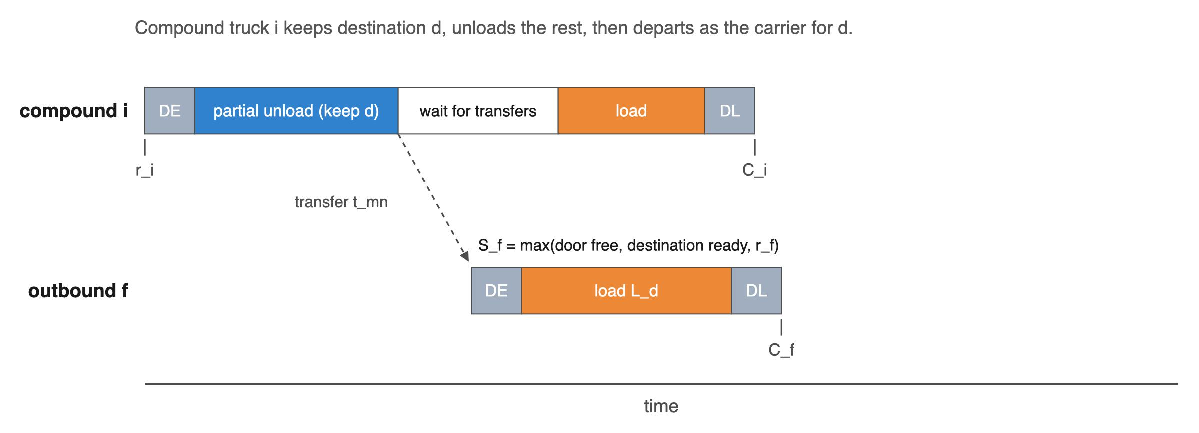
\includegraphics[width=0.92\columnwidth]{fig0_compound_timeline.pdf}
\caption{Figure 1. Processing timeline of a compound truck and the outbound truck
of its retained destination.}\label{fig:timeline}
\end{figure}

\subsection{3.2 Mixed-integer 정식화}
이진 변수 $x_{idm}$은 병행 트럭 $i\in I$를 유지 목적지 $d$·도어 $m$에,
$z_{fdm}$은 출고트럭 $f\in F$를 배정한다. $X_{im}=\sum_d x_{idm}$,
$Z_{fm}=\sum_d z_{fdm}$, $Z_{fd}=\sum_m z_{fdm}$로 두고, $b_{fgm}$은 도어 $m$에서
$f$가 $g$에 선행하면 1이다. 연속 변수 $U_i,C_i,S_f,C_f,C_{\max}$는 각각 병행 트럭의 하역 완료,
병행 트럭의 도어 작업 완료, 출고 도어 작업 시작, 출고 완료, 총 작업완료시간이다.
$L_{id}=\sum_{j\ne i}h_{jd}$, $L_d=\sum_i h_{id}$, $B$는 유효한 horizon 상한이다.

배정 제약은 다음과 같다.
\[\textstyle\sum_{d,m}x_{idm}=1\quad\forall i \qquad (1)\]
\[\textstyle\sum_{d,m}z_{fdm}=1\quad\forall f \qquad (2)\]
\[\textstyle\sum_{i,m}x_{idm}+\sum_{f,m}z_{fdm}=1\quad\forall d \qquad (3)\]
\[\textstyle\sum_{i,d}x_{idm}\le1\quad\forall m \qquad (4)\]

병행 트럭의 시간 관계와 유입 이송 선행 제약은 다음과 같다.
\[U_i=r_i+DE_i+H_i-\textstyle\sum_{d,m}h_{id}x_{idm}\quad\forall i \qquad (5)\]
\[C_i\ge U_i+L_{id}+DL_i-B(1-x_{idm})\quad\forall i,d,m \qquad (6)\]
\[C_i\ge U_j+t_{nm}+L_{id}+DL_i-B(2-x_{idm}-X_{jn}) \qquad (7)\]
식~(7)은 모든 $i,d,m,n$과 $\sum_k f_{jdk}>0$인 기여 트럭 $j\ne i$에 대해 성립한다.

출고 운송 트럭에 대해서는 다음이 성립한다.
\[S_f\ge r_f\quad\forall f \qquad (8)\]
\[C_f\ge S_f+DE_f+L_d+DL_f-B(1-Z_{fd})\quad\forall f,d \qquad (9)\]
\[S_f\ge U_i+t_{nm}-B(2-z_{fdm}-X_{in}) \qquad (10)\]
\[S_f\ge C_i-B(2-Z_{fm}-X_{im})\quad\forall f,i,m \qquad (11)\]

같은 도어 $m$을 쓰는 출고트럭 쌍 $f<g$에 대한 순서 결정과 non-overlap 제약은
다음과 같다.
\[b_{fgm}+b_{gfm}\ge Z_{fm}+Z_{gm}-1,\quad b_{fgm}\le Z_{fm},\quad b_{fgm}\le Z_{gm} \qquad (12)\]
\[S_g\ge C_f-B(1-b_{fgm}) \qquad (13)\]
\[S_f\ge C_g-B(1-b_{gfm}) \qquad (14)\]
끝으로 총 작업완료시간은 다음으로 정의된다.
\[C_{\max}\ge C_i\quad\forall i,\qquad C_{\max}\ge C_f\quad\forall f \qquad (15)\]

CP-SAT 모형은
big-$M$ disjunction을 enforcement literal로 대체하고 모든 시간값을 가장 가까운
0.01 단위로 반올림한 뒤 100배하여 정수로 변환하며, 모든 배정을 고정하면 독립
evaluator의 완료 시각이 재현되어 model fidelity가 확인된다.

\subsection{3.3 시간 제약 확장과 목적식}
각 트럭 $q\in I\cup F$는 앞서 정의한 도착 시각 $r_q\ge0$과 soft due date $\bar d_q$를 갖고
$T_q\ge\max\{0,C_q-\bar d_q\}$이다. 목적식은
\[\min\ J=C_{\max}+\lambda\sum_{q\in I\cup F}T_q,\qquad \lambda=1 \qquad (16)\]
$r_q=0$, $\bar d_q=\infty$이면 기존 총 작업완료시간 모델로 환원된다. CP-SAT는 incumbent와
증명된 하한을 함께 반환하며, 하한과 일치가 증명될 때에만 최적으로 부른다.

\subsection{3.4 조합적 하한}
CP-SAT가 제공하는 하한이 약한 실험 조건에서 격차를 보고하기 위해 도어 경합을 완화한 두 유효 하한을
사용한다. 병행 트럭 $i$(목적지 $d$ 유지)의 최속 완료와 출고트럭 $f$의 최속
완료는
\[EF_i=r_i+DE_i+\min_{d\in D}\Big(H_i-h_{id}+\textstyle\sum_{j\in I\setminus\{i\}}h_{jd}\Big)+DL_i \qquad (17)\]
\[EF_f=r_f+DE_f+\min_{d\in D}\textstyle\sum_{j\in I}h_{jd}+DL_f \qquad (18)\]
critical-chain 하한은 $LB_{\mathrm{cc}}=\max_{q\in I\cup F}EF_q$이다. door-area
하한은 각 트럭의 최소 도어 점유
\[o_i=DE_i+\Big(H_i-\max_d h_{id}\Big)+\min_d\textstyle\sum_{j\in I\setminus\{i\}}h_{jd}+DL_i \qquad (19)\]
\[o_f=DE_f+\min_d\textstyle\sum_{j\in I}h_{jd}+DL_f \qquad (20)\]
을 도어 수로 나눈 값이다.
\[LB_{\mathrm{da}}=\frac{1}{|M|}\Big(\sum_i o_i+\sum_f o_f\Big) \qquad (21)\]
두 하한 모두 제약을 완화하여 얻으므로 이들의 최댓값
$LB_\tau=\max\{LB_{\mathrm{cc}},LB_{\mathrm{da}}\}$는 총 작업완료시간의 유효 하한이다.
또한 각 $EF_q$가 $C_q$의 하한이므로 구조적 지연 하한은
\[LB_T=\sum_{q:\bar d_q<\infty}\max\{0,\ EF_q-\bar d_q\} \qquad (22)\]
이며, $LB_J=LB_\tau+\lambda LB_T$는 식 (16)의 유효 하한이다.

\section{4. 휴리스틱 알고리즘}

VAA-GILS는 iterated local search의 구현체로, 연산자 내부 sampling과 acceptance를
제외하면 결정론적이다. 이하에서 \textbf{원 모델}은 Shahmardan과
Sajadieh(2020)가 제안한 SA-RL5를 가리키며, VAA 구성 휴리스틱과
기본 이웃 7종은 이 모델에서 가져왔다.

\textbf{초기해 구성.} 원 모델의 VAA는 Vogel식 regret으로 병행 트럭의 유지 목적지를
정하고, 완료 시각 우선순위에 따라 출고 목적지를 배정한다. 도어 배정은 먼저 처리되는
트럭을 도어 간 이송시간 합이 가장 작은 중앙 도어에 두고, 나머지 트럭은 작업 종료가 가장
이른 도어에 차례로 삽입한다. 모든 완료 예정 시각 계산에는 도착 시각을 반영한다.

\textbf{Descent.} 세 가지 이동 유형(출고트럭 재배치, 병행 트럭의 도어 교환/빈 도어 이동, 두
트럭의 목적지 교환)에 대한 best-improvement 지역탐색으로, 지역 최적해(Local Optimum)에서
종료하며 초기해·모든 신규 incumbent·최종해에 적용한다.

\textbf{반복 탐색.} 1{,}000회 반복한다. 선택 정책이 연산자 하나를 뽑아
현재 해에서 후보를 생성하고, 후보가 전역 최선해를 개선하면 descent를 적용해
incumbent를 갱신한다. acceptance는 초기 온도 $T_0=\max\{1,0.05\,J(s_0)\}$, 기하
냉각 $T\leftarrow0.995\,T$의 simulated annealing이다.

\textbf{Kick restart와 reheating.} 30회 연속 개선이 없으면 \textbf{kick restart}를
수행한다. 현재 최선해 $s^*$의 복사본에서 다시 시작하되, 아래 기본 이웃 7종에서
균등 무작위로 뽑은 이동(kick)을 3회 연속 적용한다. 각 이동은 직전 이동의 결과에
적용되며, 재시작 직후에는 descent를 수행하지 않는다. 이어서
$T\leftarrow\max\{T,0.02\,J(s^*)\}$로 온도를 reheat한다.

\textbf{Operator pool.} 기본 이웃 7종은 원 모델의 이웃 구조를 그대로 사용한다:
(k1) 두 트럭의 목적지 교환, (k2) 병행 트럭 간 도어 교환, (k3) 출고트럭 간 도어
교환, (k4) 출고트럭을 다른 도어로 삽입, (k6) 하역시간 기반 룰렛 선택으로 병행 트럭을 도어에 삽입, (k7) 적재시간 기반 룰렛 선택으로 출고트럭을 도어에 삽입,
(k8) 룰렛 선택으로 병행 트럭에 목적지를 배정. 원 모델은 이동을 k1--k8로
번호매기나 k5는 정의하지 않아 실제 구현은 7종이다. 여기에 현재 병목을 먼저 식별한 뒤 그
주변에서 가능한 후보를 모두 평가해 최선을 택하는 guided 연산자 4종을 더한다: (g1) critical door의 마지막
출고트럭을 최선 도어·위치로 재배치, (g2) critical 트럭의 목적지를 전 트럭과
대조해 최선 교환, (g3)/(g4) most tardy 트럭 기준의 동일 이동(tardy인 트럭이 없으면
g1/g2로 fallback). 고속 증분 evaluator(평가당 수십 $\mu$s)가 descent와 guided 이동을
저렴하게 만든다.

\textbf{선택 정책과 원 모델의 비교.} 선택 정책은 교체할 수 있으며 기본값은
균등 무작위 선택이다. 학습 정책(SA-RL5의 tabular
Q-learning~\cite{watkins1992}, 규모 불변 특징(feature)으로 오프라인 학습한 transfer
DQN~\cite{mnih2015})은 ablation 목적으로만 평가하며 제안 방법의 일부가 아니다.
tabular Q는 원 모델과 같이 무개선 구간 5-상태에서 $\varepsilon$-greedy 탐험과 룰렛
활용을 쓰되, 보상은 원 모델의 이진 보상(후보가 현재 해보다 나쁘지 않으면 1, 아니면 0)
대신 신규 incumbent 2·비악화 1·그 외 0의 셰이핑 보상을 사용한다. 이는 학습 신호를
강화할 뿐이므로 비교 대상 선택 정책을 불리하게 만들지 않는다. 원 모델 SA-RL5는 RL이 단일 이동을 고르고 SA accept/reject로 한 단계가 끝나는
\textbf{순수} simulated annealing인 반면, VAA-GILS는 그 한 연산자 적용 단계를 iterated
local search 안에 넣고 guided 연산자, 개선 이동마다의 full descent, kick
restart를 더한다. 가장 중요한 차이는 개선 이동 이후의 descent이며, ablation은
이것이 품질 이득의 대부분을 설명함을 보인다. 두 방법의 구조적 차이는
<Table~
ef{tab:base}>에 정리하였다.

\begin{table}[H]\centering
\caption{Table 1. Structural comparison of the base SA-RL5 and VAA-GILS.}
\label{tab:base}\small
\begin{tabular}{@{}p{0.24\columnwidth}p{0.33\columnwidth}p{0.33\columnwidth}@{}}
\toprule
Aspect & SA-RL5 (base) & VAA-GILS (proposed) \\
\midrule
Overall framework & Pure simulated annealing & Iterated local search (SA only as acceptance) \\
Operators per iteration & One & One (same) \\
Operator set & 7 generic neighborhoods & Those 7 + 4 guided \\
Operator selection & Online Q-learning / roulette & Uniform random (learning only in ablation) \\
After an improving move & None (the SA step is the whole iteration) & Full best-improvement descent \\
Stagnation handling & None & Kick restart + reheating \\
Acceptance & SA (Metropolis) & SA (Metropolis; dispensable per ablation) \\
Objective & Makespan & Makespan + λ · total 납기지연 \\
\bottomrule
\end{tabular}
\end{table}

\section{5. 실험 설계}

\subsection{5.1 인스턴스 생성}
병행 트럭 $|I|$, 출고트럭 $|F|$, 목적지 $|D|=|I|+|F|$, 도어 $|M|=|I|$로 두고 세 규모를
사용한다: S $(|I|,|F|)=(6,3)$, M $(12,6)$, L $(20,10)$. 따라서 $(|I|,|D|,|M|)$는 각각
$(6,9,6)$, $(12,18,12)$, $(20,30,20)$이고 병행 트럭 비율 $|I|/|D|$는 모두 $2/3$이다. S는
CP-SAT가 제한시간 안에 최적성을 증명할 수 있는 규모이고 L은 실행 가능해조차 얻기 어려운
규모여서 두 극단을 함께 본다. 병행 트럭 비율을 높게 잡은 것은, 이 비율이 낮으면 문제가
일반 크로스도킹 스케줄링에 가까워져 부분 하역 구조의 영향이 드러나지 않기 때문이다.

나머지 생성 파라미터는 <Table~\ref{tab:param}>에 정리하였다. 화물이 특정 목적지로
쏠리는 정도는 이와 별개의 조건이며, 보고하는 모든 실험은 쏠림이 없는 조건을 사용한다(쏠린
조건과 군집 조건은 부록 A의 transfer DQN 학습에만 쓴다). 도어를 일렬로 늘어놓으면
이송시간이 도어 번호 차이로 정해져 도어 배정이 해에 미치는 영향이 작아지므로, 배정
결정이 실제로 품질을 가르도록 무작위 배치를 쓴다. 이송 거리를 10으로 나누는 것은
이송시간을 처리시간과 같은 크기 범위에 두기 위해서다.

\begin{table}[H]\centering
\caption{Table 2. Instance generation parameters. Flow, handling and
enter/leave times are drawn from integer uniform distributions.}
\label{tab:param}\small
\begin{tabular}{@{}llp{0.40\columnwidth}@{}}
\toprule
Item & Symbol & Value \\
\midrule
Size (compound/outbound/destination/door) & $(|I|,|F|,|D|,|M|)$ & S $(6,3,9,6)$; M $(12,6,18,12)$; L $(20,10,30,20)$ \\
Compound-truck ratio & $|I|/|D|$ & $2/3$ \\
Number of product types & $|K|$ & 3 \\
Flow & $f_{idk}$ & $U[0,20]$ \\
Unit handling time & $t_k$ & $U[1,4]$ \\
Enter/leave time & $DE_q,DL_q$ & $U[1,5]$ \\
Door coordinates & --- & uniform on $[0,100]^2$ \\
Inter-door travel time & $t_{mn}$ & Euclidean distance $/\,10$ \\
Release time & $r_q$ & none: $0$; otherwise $U[0,\rho H]$ \\
Soft due date & $\bar d_q$ & none: $\infty$; otherwise $r_q+\delta H$ \\
Time-constraint level & $(\rho,\delta)$ & medium $(0.25,0.60)$; tight $(0.50,0.35)$ \\
\bottomrule
\end{tabular}
\end{table}

\subsection{5.2 시간 제약 수준}
시간 제약은 none, medium, tight 세 수준이다. none은 $r_q=0$, $\bar d_q=\infty$로 두어
모든 트럭이 시각 0에 가용하고 납기가 없는 기존 모델과 같으며, 본 연구의 확장을 껐을 때의
대조군 역할을 한다. medium과 tight에서는 $r_q\sim U[0,\rho H]$, $\bar d_q=r_q+\delta H$,
$(\rho,\delta)=(0.25,0.60),(0.50,0.35)$이다. 여기서 $H=2\sum_{i\in I}H_i/|M|$는 시간
제약이 없을 때의 총 작업완료시간 추정치로, 화물 한 단위가 하역과 적재로 두 번 처리되므로
계수 2를 둔다. 시간 제약을 $H$의 비율로 주면 규모가 달라져도 압박 수준이 유지된다.
$\rho$는 도착이 퍼지는 폭, $\delta$는 도착 후 납기까지의 여유를 뜻하므로, tight는 두
방향으로 동시에 어려워지는 조건이다.

규모 3종과 시간 제약 3수준을 교차해 총 9개의 실험 조건을 만들고, 각 조건을 S-none,
M-tight와 같이 규모-수준 형태로 표기한다.

\subsection{5.3 비교 대상과 측정}
비교 대상은 다섯이다. (i) VAA는 구성 휴리스틱만 적용한 초기해, (ii) Paper-SA-RL5는 원
모델의 재구현이며, (iii)--(v) GILS-uniform, GILS-tabular, GILS-DQN은 선택 정책만 바꾼 제안
방법의 세 변형이다. 제안 방법의 기본값은 GILS-uniform이고 나머지 두 변형은 학습 기반
선택의 효과를 보기 위한 것이다. 여기에 CP-SAT 결과를 함께 보고한다. 원 모델은 도착
시각과 납기를 다루지 않으므로 Paper-SA-RL5는 none 조건에서만 비교한다.

인스턴스 seed는 학습·조정·시험 세 집합으로 서로소가 되게 나눈다. 학습 정책은 학습
집합에서만 훈련하고 $\lambda$와 같은 설계 값은 조정 집합에서만 고르므로 시험 집합의
성능이 부풀려지지 않는다. 주 해품질 비교(<Table~\ref{tab:main}>)는 조건당 시험 인스턴스
20개를 각각 5회 반복 실행한다. 인스턴스마다 난이도가 다르므로 여러 개가 필요하고,
알고리즘에 무작위성이 있으므로 같은 인스턴스도 여러 번 실행한다. 통제된
ablation(<Table~\ref{tab:b1}>--<Table~\ref{tab:sel}>)은 같은 엔진에서 구성요소만 떼어내는
짝지은 비교여서 인스턴스 간 난이도 편차가 상쇄되므로 조건당 5개만 사용한다.

같은 인스턴스의 5회 반복은 서로 독립이 아니므로, 먼저 인스턴스별로 평균해 조건당 값
하나를 만든 뒤 짝지은 인스턴스 평균에 양측 Wilcoxon signed-rank test를 적용한다. 주
지표는 인스턴스별 격차 $\Delta_{bo}$이며, 해당 인스턴스에 대해 모든 방법과 모든 반복
횟수, CP-SAT 결과까지 통틀어 관측된 가장 좋은 목적값을 기준으로 삼는다. 대형 조건에서는
CP-SAT 기준해가 없어 최적해 대비 갭을 쓸 수 없기 때문이다.

GILS 계열의 종료 조건은 반복 횟수 1{,}000회로 통일한다. CP-SAT는 인스턴스당 1회, 8
thread로 S에 300초(5개), M과 L에 600초(조건당 2개)를 부여하며 S-none 5개에서만 최적성이
증명된다. 실험은 Apple M2 칩(8코어)과 16\,GB 메모리를 갖춘 macOS 환경에서 Python 3.12와 OR-Tools 9.15로 수행하였다.

\section{6. 실험 결과}
\subsection{6.1 해 품질}
<Table~
ef{tab:main}>에 20개 인스턴스에 대한 시험 결과를 요약한다. CP-SAT가 기준해를 제공한
실험 조건에서 GILS는 이에 근접하며, 기본 선택 정책인 균등 선택 기준 0.11--0.21\%이다
(학습 선택 정책을 포함한 전체 변형은 0.1--0.6\%). 같은 선택 정책 기준으로 GILS는
VAA를 평균 2.65\%($n=180$, $p<10^{-4}$), SA-RL5를 1.38\%($n=60$, $p<10^{-4}$)
능가한다. 실행 시간은 S/M/L에서 각각 0.11, 0.52, 2.3초로, 같은 조건의
CP-SAT(76, 237, 376초)보다 두세 자릿수 짧다.

\begin{table}[t]\centering
\caption{Table 3. Test results over 20 instances per experimental condition (20 instances $\times$ 5 replications). $\Delta_{bo}$ is the mean gap to the best observed solution and time is the mean per run. The vs CP-SAT column is computed only on the subset for which CP-SAT returned a reference (5 instances per S condition, 2 for M-none); optimality was proven only for S-none. On that subset the mean CP-SAT runtime is 76 s (S) and 237 s (M-none).}
\label{tab:main}\small
\begin{tabular}{@{}llrrrr@{}}
\toprule
Condition & Method & Mean obj. ± s.d. & Δbo(\%) & vs CP-SAT(\%) & Time(s)\\
\midrule
S-none & VAA & 1497.5 ± 400.3 & 6.60 & +6.49 & 0.00\\
 & Paper-SA-RL5 & 1423.3 ± 383.6 & 1.03 & +1.21 & 0.15\\
 & GILS-uniform & 1411.8 ± 382.7 & 0.16 & +0.21 & 0.08\\
 & GILS-tabular & 1412.9 ± 381.3 & 0.28 & +0.33 & 0.11\\
 & GILS-DQN & 1416.1 ± 382.4 & 0.51 & +0.75 & 0.23\\
S-medium & VAA & 5447.5 ± 1468.9 & 3.89 & +3.33 & 0.00\\
 & GILS-uniform & 5255.7 ± 1413.3 & 0.08 & +0.11 & 0.08\\
 & GILS-tabular & 5259.1 ± 1412.3 & 0.15 & +0.18 & 0.11\\
 & GILS-DQN & 5270.8 ± 1415.3 & 0.38 & +0.55 & 0.22\\
S-tight & VAA & 9276.8 ± 2387.6 & 2.90 & +2.17 & 0.00\\
 & GILS-uniform & 9010.8 ± 2206.1 & 0.09 & +0.21 & 0.09\\
 & GILS-tabular & 9011.9 ± 2206.7 & 0.11 & +0.17 & 0.11\\
 & GILS-DQN & 9022.0 ± 2205.3 & 0.23 & +0.34 & 0.22\\
M-none & VAA & 3030.9 ± 903.6 & 3.73 & +4.80 & 0.00\\
 & Paper-SA-RL5 & 2976.4 ± 864.4 & 1.86 & +0.99 & 0.55\\
 & GILS-uniform & 2928.9 ± 842.6 & 0.29 & +0.13 & 0.43\\
 & GILS-tabular & 2932.1 ± 846.3 & 0.37 & +0.11 & 0.52\\
 & GILS-DQN & 2932.5 ± 845.5 & 0.40 & +0.19 & 0.73\\
M-medium & VAA & 23025.5 ± 4075.4 & 2.56 & --- & 0.00\\
 & GILS-uniform & 22526.4 ± 3960.5 & 0.29 & --- & 0.44\\
 & GILS-tabular & 22515.5 ± 3964.0 & 0.24 & --- & 0.55\\
 & GILS-DQN & 22540.3 ± 3956.4 & 0.36 & --- & 0.75\\
M-tight & VAA & 38903.7 ± 11283.5 & 1.25 & --- & 0.01\\
 & GILS-uniform & 38528.0 ± 11078.0 & 0.19 & --- & 0.48\\
 & GILS-tabular & 38512.1 ± 11059.5 & 0.16 & --- & 0.60\\
 & GILS-DQN & 38543.6 ± 11077.6 & 0.24 & --- & 0.81\\
L-none & VAA & 5492.3 ± 1482.2 & 2.21 & --- & 0.02\\
 & Paper-SA-RL5 & 5479.7 ± 1449.5 & 1.97 & --- & 1.92\\
 & GILS-uniform & 5388.4 ± 1427.3 & 0.27 & --- & 2.16\\
 & GILS-tabular & 5385.5 ± 1424.6 & 0.22 & --- & 2.54\\
 & GILS-DQN & 5386.1 ± 1425.2 & 0.23 & --- & 2.99\\
L-medium & VAA & 55611.1 ± 18087.3 & 1.52 & --- & 0.02\\
 & GILS-uniform & 54846.4 ± 17523.5 & 0.10 & --- & 2.10\\
 & GILS-tabular & 54833.4 ± 17526.8 & 0.07 & --- & 2.52\\
 & GILS-DQN & 54848.8 ± 17522.9 & 0.11 & --- & 2.85\\
L-tight & VAA & 119671.9 ± 32475.3 & 0.77 & --- & 0.02\\
 & GILS-uniform & 118901.4 ± 31781.1 & 0.08 & --- & 2.01\\
 & GILS-tabular & 118865.6 ± 31788.4 & 0.05 & --- & 2.51\\
 & GILS-DQN & 118888.8 ± 31789.1 & 0.07 & --- & 2.76\\
\bottomrule
\end{tabular}
\end{table}

\subsection{6.2 핵심 구성요소 분석: 성능은 어디에서 오는가}
세 가지 통제된 ablation(반복 횟수 1{,}000회 고정)으로 엔진을 분해한다.

\textbf{Operator pool.} 선택 정책을 균등 선택으로 고정하고 연산자 집합만 기본(7종)/
핵심(+g1,g2)/전체(+g3,g4)로 바꾸면 $\Delta_{bo}$가 9개 실험 조건 전부에서
기본 $\ge$ 핵심 $\ge$ 전체로 단조 감소한다(<Figure~\ref{fig:op}>). 짝지은
Wilcoxon(<Table~\ref{tab:b1}>)은 유도 연산자가 목적값을 일관되게·유의하게 낮춤을
보인다.

\begin{table}[H]\centering
\caption{Table 4. Operator-pool ablation (5 instances $\times$ 5 replications per condition, the number of iterations fixed at 1,000; two-sided Wilcoxon, positive mean favors the richer operator set).}
\label{tab:b1}\small
\begin{tabular}{@{}lrrl@{}}
\toprule
Contrast & n & Gain(\%p) & p\\
\midrule
generic → critical (add g1, g2) & 136 & +0.114 & <0.0001\\
critical → full (add g3, g4) & 172 & +0.048 & <0.0001\\
generic → full (all guided) & 166 & +0.161 & <0.0001\\
\bottomrule
\end{tabular}
\end{table}

\begin{figure}[H]\centering
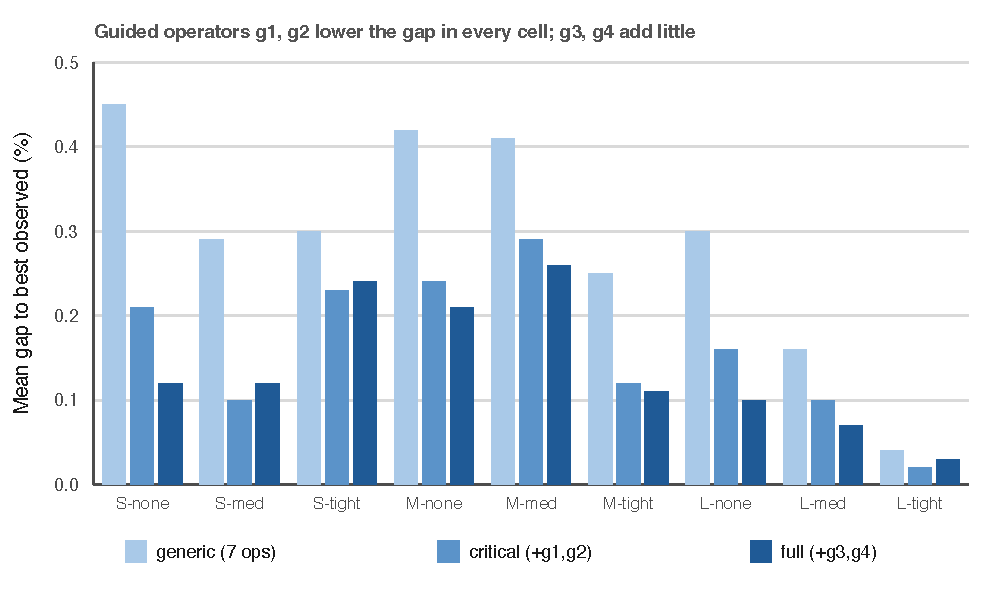
\includegraphics[width=0.82\columnwidth]{fig2_operator_pool.pdf}
\caption{Figure 2. Mean gap to the best observed solution by operator set.}\label{fig:op}
\end{figure}

\textbf{Engine components.} 연산자 집합을 전체로, 선택 정책을 균등 선택으로 고정하고 구성요소를
하나씩 제거하면(<Table~\ref{tab:b2}>), best-improvement descent의 기여가 가장 크고 kick
restart가 그다음이며, VAA 초기해는 통계적으로 유의하지 않고 확률적 acceptance는
제거해도 목적값이 나빠지지 않는다(<Figure~\ref{fig:comp}>).

\begin{table}[H]\centering
\caption{Table 5. Engine-component ablation (5 instances $\times$ 5 replications per condition; leave-one-out, relative objective degradation when a component is removed).}
\label{tab:b2}\small
\begin{tabular}{@{}lrrl@{}}
\toprule
Removed component & n & Degradation(\%p) & p\\
\midrule
best-improvement descent & 45 & +0.156 & <0.0001\\
kick restart & 43 & +0.069 & <0.0001\\
VAA initial solution & 45 & +0.022 & 0.114\\
stochastic acceptance & 45 & −0.026 & 0.0014\\
\bottomrule
\end{tabular}
\end{table}

\begin{figure}[H]\centering
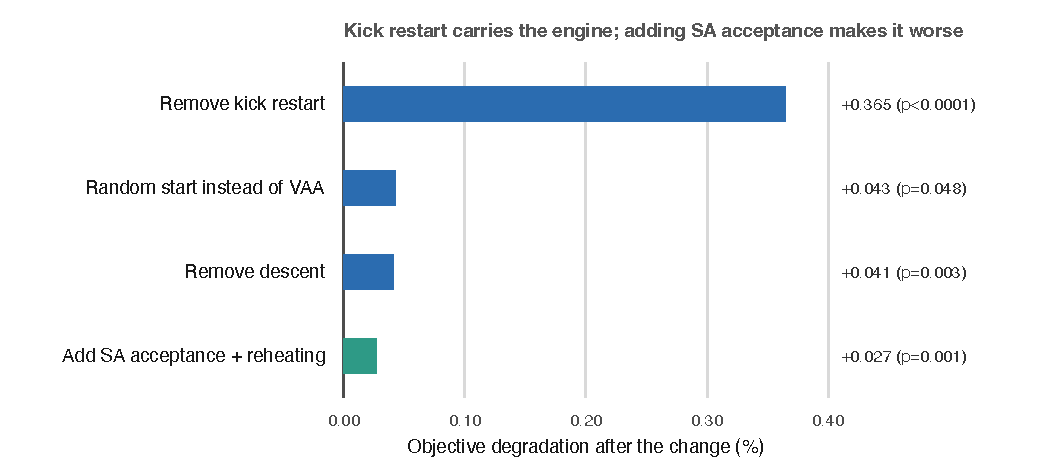
\includegraphics[width=0.82\columnwidth]{fig3_component_ablation.pdf}
\caption{Figure 3. Objective degradation when each component is removed.}\label{fig:comp}
\end{figure}

\subsection{6.3 보조 분석: 학습 기반 연산자 선택}
연산자 집합과 구성요소를 전체로 고정하고 선택 정책만 바꾸면(<Table~\ref{tab:sel}>), 어떤
학습 정책도 균등 선택을 실용적으로 능가하지 못한다. 반복 횟수를 50--3{,}000회로 바꾸어도 결과는 같고 우열의 방향이
반복 횟수에 따라 뒤집히며(<Figure~\ref{fig:sel}>),
이러한 부정적 결과는 무제약 조건만으로도 성립하므로 시간 제약 확장 때문에 나타난
결과가 아니다.

\begin{table}[H]\centering
\caption{Table 6. Effect of the selection policy (5 instances $\times$ 5 replications per condition, 1,000 iterations; two-sided Wilcoxon, positive mean favors the first method).}
\label{tab:sel}\small
\begin{tabular}{@{}lrrl@{}}
\toprule
Comparison & Mean diff.(\%p) & p & Verdict\\
\midrule
tabular vs uniform & −0.01 & 0.150 & No difference\\
tabular vs DQN & +0.10 & <0.0001 & DQN worse\\
uniform vs DQN & +0.11 & <0.0001 & DQN worse\\
\bottomrule
\end{tabular}
\end{table}

\subsection{6.4 Tardiness-weight 민감도}
식 (16)이 시간 단위 성분 둘을 합치므로 조정 집합에서
$\lambda\in\{0,0.25,0.5,1,2,4,8\}$을 스윕한다. 물리적 총 작업완료시간과 총 납기지연을
인스턴스별로 min--max 정규화해 평균한다(<Figure~\ref{fig:lam}>). 납기지연 감소의
대부분은 $\lambda=0$에서 $1$ 사이에서 일어나고 이후에는 그 폭이 줄어든다. 전체 스윕 구간에서 평균
총 작업완료시간은 약 1\% 상승, 평균 납기지연은 2--3\% 하락한다. $\lambda=1$을 채택한다:
완만한 총 작업완료시간 비용으로 납기지연이 거의 최소에 이르고 두 시간 성분에 동일
가중을 준다. 이 스윕은 시험이 아닌 조정 인스턴스를 사용한 설계 정당화이다.

\begin{figure}[H]\centering
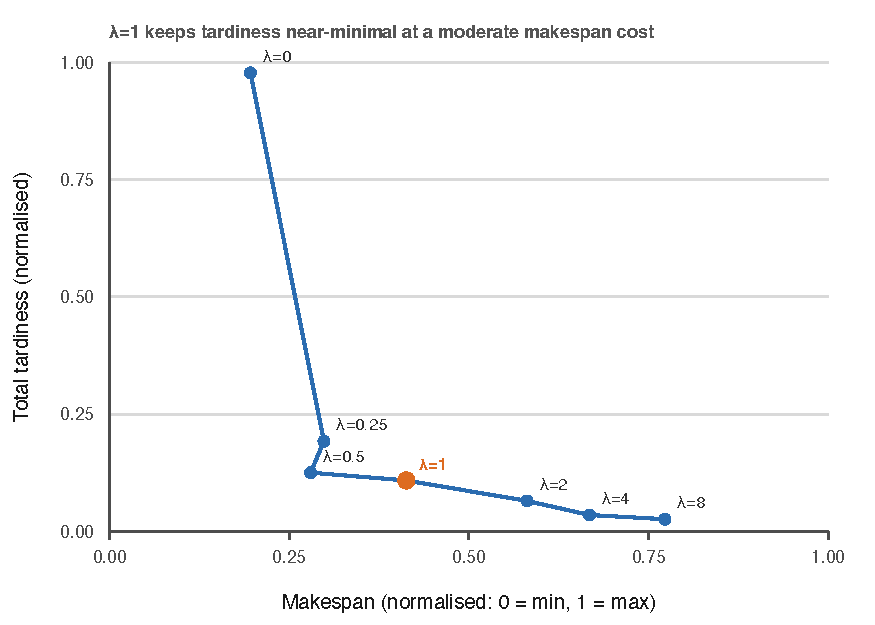
\includegraphics[width=0.72\textwidth]{fig4_lambda_tradeoff.pdf}
\caption{Figure 4. Normalized makespan-tardiness trade-off on tuning instances.}\label{fig:lam}
\end{figure}

\section{7. 논의}
학습 기반 선택 정책이 균등 선택 대비 이득을 주지 못한 것은 학습 일반에 대한 결론이
아니라 본 논문의 탐색 구조가 낳은 결과다. 후보 하나의 평가에 수십 $\mu$s밖에 들지
않아 연산자를 잘 고르는 것보다 많이 시도하는 편이 유리하고, 모든 신규 최선해 뒤에
결정론적 descent가 따라붙어 어떤 연산자로 그 지점에 이르렀는지의 차이를 상당 부분
흡수한다. 반복 횟수별 격차 곡선도 대부분의 시험 인스턴스에서 해 품질이 1{,}000회 이전에
평탄해짐을 보인다. SA acceptance와 reheating은 원 모델과 비교할 수 있도록
유지하였으나, ablation은 본 설정에서 이 둘이 해 품질에 필수적이지 않음을 보인다.

선택 정책이 예측할 대상이 마땅치 않다는 점도 작용한다. 본 문제의 인스턴스는 정적이고
모든 도착 시각이 최적화 이전에 알려져 있어, 실행 도중 새로 드러나 정책이 활용할
정보가 없다. 도착 정보가 시간에 따라 공개되는 동적 도크 운영이나 이동 하나의 평가가
비싼 시뮬레이션 기반 모형에서는 판단이 달라질 수 있다. 따라서 본 결과의 함의는 학습이
무용하다는 것이 아니라 비교 조건에 있다. 학습 기반 선택 정책은 동일한 엔진과 동일한
반복 횟수 아래 균등 선택과 견주어야 하며, 그 통제가 없으면 descent·restart·강한
연산자 집합의 이득이 정책의 성과로 잘못 귀속될 수 있다.

\section{8. 결 론}
본 연구는 부분 하역 병행 트럭 스케줄링에 도착 시각과 soft due date를
도입하고, MILP·CP-SAT 정식화와 유효 하한으로 휴리스틱 해를 검증하였다. CP-SAT
기준해가 있는 실험 조건에서 VAA-GILS의 목적값은 해당 기준해 대비 평균 0.11--0.21\%였고(소형 무제약
조건에서는 CP-SAT가 최적성을 증명하였다), 대형 시간 제약 조건에서는 수 초 안에 비교 방법 가운데 가장 좋은 해를 제공하였다.
ablation은 성능이 best-improvement descent, guided 이동, restart라는 결정론적
구조에서 비롯되며, 학습 기반 연산자 선택·학습된 초기해·확률적 acceptance는 이
환경에서 실용적 이득을 주지 않음을 보였다. 향후에는 도착 정보가 실시간으로 공개되는 동적
문제, 대형 시간 제약 조건을 위한 더 강한 하한, 산업 데이터를 활용한 사례 연구가 필요하다.

\appendix
\section{부록 A. Transfer DQN 구현 세부}
transfer DQN은 매 반복 11개 연산자 집합에서 하나를 고른다. Q-network는 27차원 규모
불변 상태를 연산자별 Q값으로 사상하는 MLP로, 64 unit의 hidden layer 2개와 ReLU를
쓴다. 학습은 용량 100{,}000의 replay buffer를 사용하며, 500 transition warm-up 후
매 step 1회 gradient step으로 Huber(smooth-$L_1$) temporal-difference loss를 Adam
(learning rate $10^{-3}$, discount $\gamma=0.9$)으로 최소화한다. mini-batch는 64,
target network는 500 step마다 동기화한다. reward는 shaped signal(신규 incumbent 2,
비악화 1, 그 외 0)이다. agent는 \emph{학습} 집합(S/M 규모, 모든 화물 분포·시간 제약 조건)에서 500회
실행으로 오프라인 학습($\varepsilon$-greedy) 후, \emph{시험} 인스턴스에 zero-shot
($\varepsilon=0$, 갱신 없음)으로 적용한다. 결과가 균등 선택 대비 개선이 없다는
것이므로, 재현·강화가 가능하도록 network·학습 스크립트·seed를 공개한다.

\begin{figure}[H]\centering
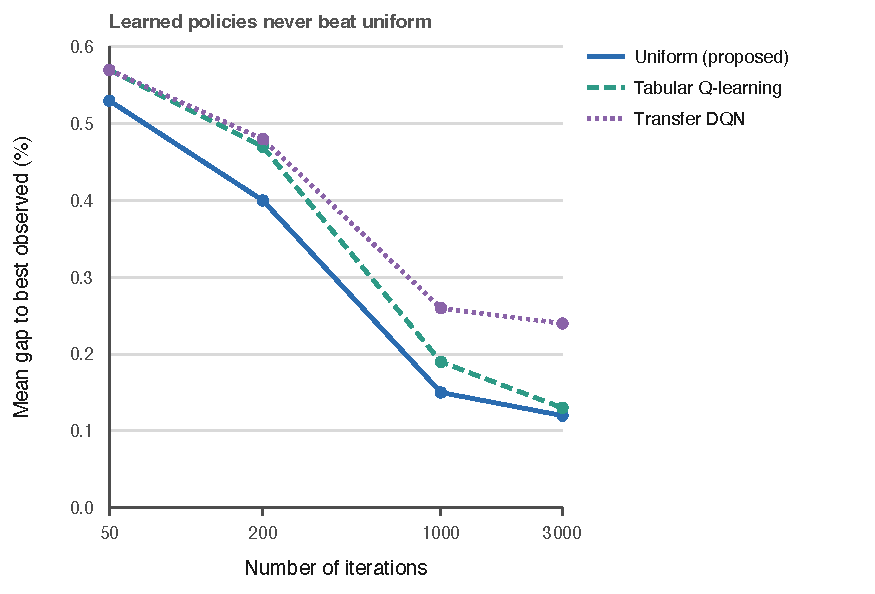
\includegraphics[width=0.72\textwidth]{fig1_selector_budget.pdf}
\caption{Figure 5. Mean gap to the best observed solution versus the number of iterations.}\label{fig:sel}
\end{figure}

\section*{생성형 AI 활용 공개}
본 논문의 작성 과정에서 저자는 OpenAI Codex(GPT-5, OpenAI)와 Claude Code(Anthropic)를
본문의 맞춤법 및 가독성 개선을 위해 사용하였다. 저자는 해당 도구 사용 후 그 내용을
검토 및 수정하였으며, 논문의 모든 내용에 대한 책임은 저자에게 있다.

\section*{참고문헌}
\begin{description}\small
\item Assadi, M. T. and Bagheri, M.(2016), Differential Evolution and Population-Based Simulated Annealing for Truck Scheduling Problem in Multiple Door Cross-Docking Systems, \emph{Computers \& Industrial Engineering}, 96, 149-161.
\item Bodnar, P., de Koster, R., and Azadeh, K.(2017), Scheduling Trucks in a Cross-Dock with Mixed Service Mode Dock Doors, \emph{Transportation Science}, 51(1), 112-131.
\item Boysen, N. and Fliedner, M.(2010), Cross Dock Scheduling: Classification, Literature Review and Research Agenda, \emph{Omega}, 38(6), 413-422.
\item Joo, C. M. and Kim, B. S.(2013), Scheduling Compound Trucks in Multi-Door Cross-Docking Terminals, \emph{International Journal of Advanced Manufacturing Technology}, 64, 977-988.
\item Konur, D. and Golias, M. M.(2013a), Analysis of Different Approaches to Cross-Dock Truck Scheduling with Truck Arrival Time Uncertainty, \emph{Computers \& Industrial Engineering}, 65(4), 663-672.
\item Konur, D. and Golias, M. M.(2013b), Cost-Stable Truck Scheduling at a Cross-Dock Facility with Unknown Truck Arrivals: A Meta-Heuristic Approach, \emph{Transportation Research Part E}, 49(1), 71-91.
\item Ladier, A.-L. and Alpan, G.(2016), Robust Cross-Dock Scheduling with Time Windows, \emph{Computers \& Industrial Engineering}, 99, 16-28.
\item Larbi, R., Alpan, G., Baptiste, P., and Penz, B.(2011), Scheduling Cross Docking Operations under Full, Partial and No Information on Inbound Arrivals, \emph{Computers \& Operations Research}, 38(6), 889-900.
\item Li, Y., Mohammadi, M., Zhang, X., Lan, Y., and van Jaarsveld, W.(2026), Integrated Trucks Assignment and Scheduling Problem with Mixed Service Mode Docks, \emph{European Journal of Operational Research}, 333(1), 117-137.
\item Mnih, V., Kavukcuoglu, K., Silver, D., Rusu, A. A., Veness, J., Bellemare, M. G., Graves, A., Riedmiller, M., Fidjeland, A. K., Ostrovski, G., Petersen, S., Beattie, C., Sadik, A., Antonoglou, I., King, H., Kumaran, D., Wierstra, D., Legg, S., and Hassabis, D.(2015), Human-Level Control through Deep Reinforcement Learning, \emph{Nature}, 518, 529-533.
\item Molavi, D., Shahmardan, A., and Sajadieh, M. S.(2018), Truck Scheduling in a Cross Docking Systems with Fixed Due Dates and Shipment Sorting, \emph{Computers \& Industrial Engineering}, 117, 29-40.
\item Rijal, A., Bijvank, M., and de Koster, R.(2019), Integrated Scheduling and Assignment of Trucks at Unit-Load Cross-Dock Terminals with Mixed Service Mode Dock Doors, \emph{European Journal of Operational Research}, 278(3), 752-771.
\item Shahmardan, A. and Sajadieh, M. S.(2020), Truck Scheduling in a Multi-Door Cross-Docking Center with Partial Unloading: Reinforcement Learning-Based Simulated Annealing Approaches, \emph{Computers \& Industrial Engineering}, 139, 106134.
\item Van Belle, J., Valckenaers, P., and Cattrysse, D.(2012), Cross-Docking: State of the Art, \emph{Omega}, 40(6), 827-846.
\item Van Belle, J., Valckenaers, P., Vanden Berghe, G., and Cattrysse, D.(2013), A Tabu Search Approach to the Truck Scheduling Problem with Multiple Docks and Time Windows, \emph{Computers \& Industrial Engineering}, 66(4), 818-826.
\item Watkins, C. J. C. H. and Dayan, P.(1992), Q-Learning, \emph{Machine Learning}, 8, 279-292.
\item Xi, X., Liu, C., Wang, Y., and Lee, L. H.(2020), Two-Stage Conflict Robust Optimization Models for Cross-Dock Truck Scheduling Problem under Uncertainty, \emph{Transportation Research Part E}, 144, 102123.
\end{description}


\end{document}
